% !TeX root = Bericht.tex
% !TeX spellcheck = de_DE
\section{Durchführung}
\noindent Die Pumpe zur Evakuierung des Kryostats wurde bereits vor Eintreffen durch den Betreuer eingeschaltet. Der Aufbau des Kryostats mit den Magnetspulen zur Bestimmung des Hallkoeffizienten ist in \autoref{ExperimetAufbau} zu sehen.  Zu Beginn des Versuchs muss das Magnetfeld mithilfe eines Teslameters kalibriert werden.

\begin{figure}[H]
    \centering
    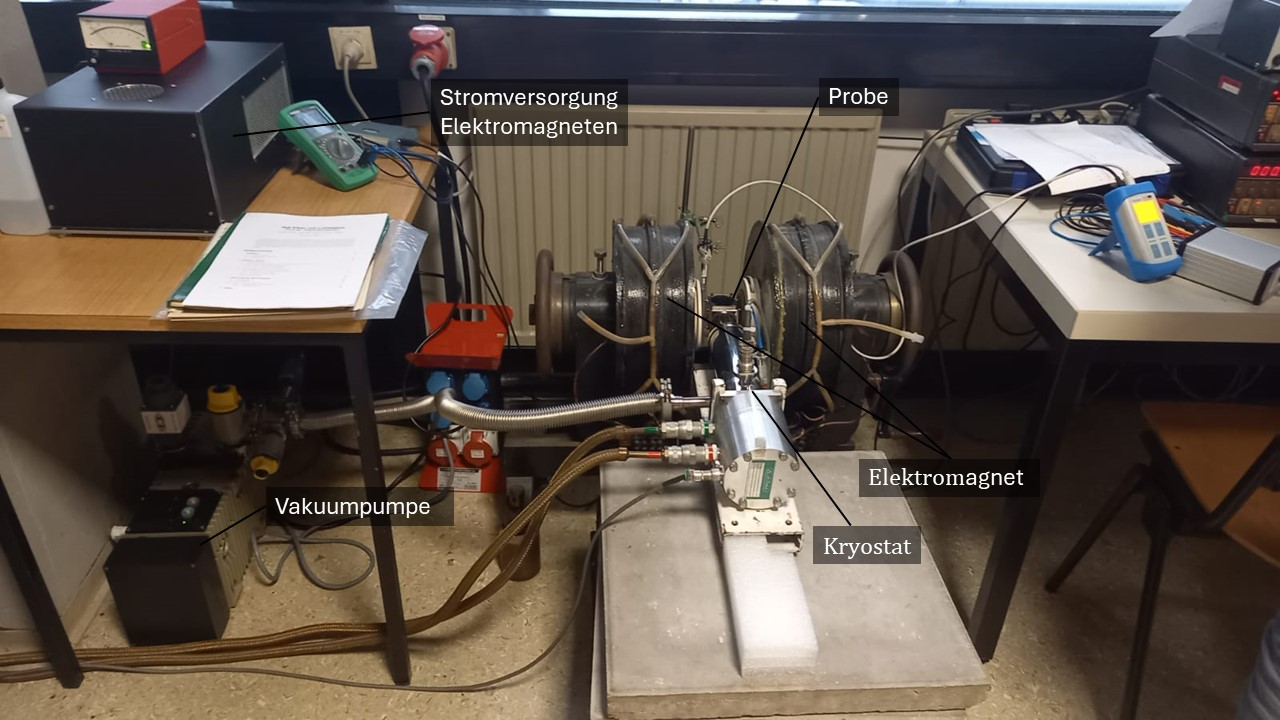
\includegraphics[width=\linewidth]{BildExberimentAufbauBeschriftung.JPG}
    \caption{In dieser Abbildung sind der Kryostat, die Magnetspulen sowie die Sonde zur Messung des Magnetfeldes zu erkennen.}
    \label{ExperimetAufbau}
\end{figure}

Dafür wird am Computer eine Magnetfeldstärke eingestellt. Da diese nicht mit der tatsächlichen Magentfeldstärke übereinstimmt, muss diese mit einem Teslameter überprüft werden.
Bei eingeschaltetem Magnetfeld sollen ungefähr $250 \unit{mT}$ an der Probe anliegen. Dies erreichen wir, indem $190 \unit{mT}$ am Computer einstellt werden.
Zudem überprüfen wir das Teslameter, wenn am Computer ein Magnetfeld von \SI{0}{mT} eingestellt wird, da auch dann aufgrund der Polarisierung des Ferromagneten ein geringes Magnetfeld erzeugt wird.
Danach wird am Netzteil eine Stromstärke von \SI{500}{\micro A} angelegt, welche über den gesamten Versuch nicht mehr verändert wird.
Als Erstes wenden wir die \blockquote{van-der-Pauw}-Methode, die in \autoref{theorie} beschrieben wird, bei Raumtemperatur an und es werden acht Spannungen gemessen.
Die einzelnen Schaltungen der \blockquote{van der Pauw}-Methode müssen nicht selbst verkabelt werden, sondern können durch Drehen eines Drehschalters realisiert werden.
Der Drehschalter ist in \autoref{drehschalter} abgebildet und die Bedeutung der Möglichkeiten des Schalters sind in \autoref{schaltungen} gezeigt.

\begin{figure}[H]
    \centering
    \includegraphics[ height=5cm]{drehschalter.jpg}
    \caption{Zu sehen ist der Drehschalter zur Realisierung der verschiedenen Schaltungen.}
   \label{drehschalter}
\end{figure}

Für die Bestimmung des spezifischen Widerstands und des Hall-Koeffizienten wird die Spannung bei den Optionen 1a, 1b, 2a, 2b, 3a und 3b gemessen, wobei das Magnetfeld ausgeschaltet ist. Dann wird das Magnetfeld aktiviert, und die Spannung erneut bei 3a und 3b gemessen.
Zudem muss die Temperatur aufgezeichnet werden.
Die Temperatur wird nicht direkt gemessen, sondern durch einen Pt100-Widerstand mit einer Vierleitermessung bestimmt.
Die Umrechnung von Widerstand in Temperatur wird in \autoref{theorie} erläutert.
Die Messung des Widerstands wird am Multimeter durchgeführt.

Nach der Messung bei Raumtemperatur wird die Temperatur abgesenkt. Während der Abkühlung werden laufend Spannungsmessungen mit selbigen Einstellungen wie bei Raumtemperatur gemacht, wobei auch die Temperatur aufgezeichnet wird.
Die Widerstandsmessung wird immer vor einer Spannungsmessung mit 1a Einstellung und nach 2a gemacht.
Hier sind zwei Temperaturmessungen zur Fehlerabschätzung hilfreich, da die Temperatur phasenweise sehr schnell sinkt.
Diese Messungen werden laufend gemacht, bis die Temperatur ihr Minimum erreicht.
Um sinnvolle Messungen zu realisieren, kann eine Heizung zugeschaltet werden, um das Abkühlen etwas zu verlangsamen.
Dies wurde in der zweiten Hälfte der Abkühlphase gemacht. Dieser gesamte Aufbau ist in \autoref{fig:BildGanz} zu erkennen.
Zuletzt wird nochmals überprüft, welchen Wert das Teslameter bei Anlegen einer Magnetfeldstärke von \SI{0}{mT} und \SI{190}{mT} anzeigt, um zu Prüfen, ob sich diese Werte während des Versuchs durch Polarisierung des Ferromagneten geändert haben.

\begin{figure}[H]
    \centering
    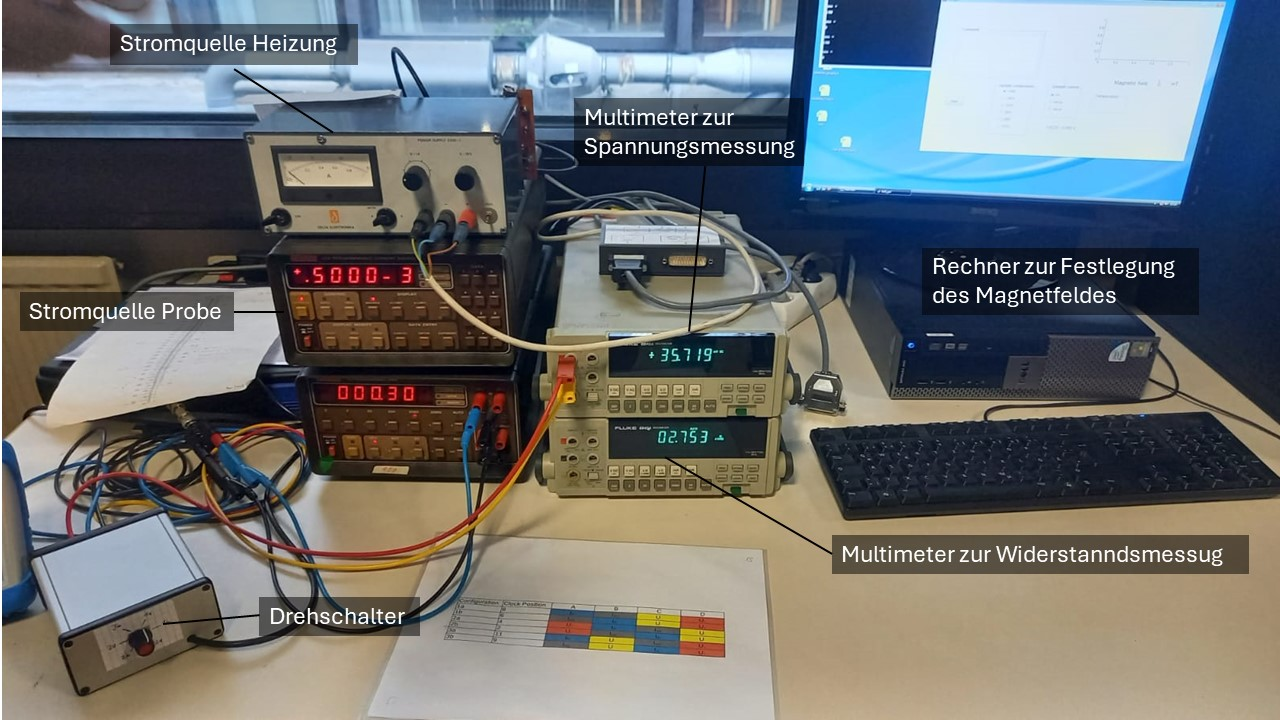
\includegraphics[width=\textwidth]{BildMitBeschriftung_Tisch.JPG}
    \caption{In dieser Abbildung ist die Stromversorgung für die Messung und die Multimeter zur Bestimmung des Widerstandes im PT100 und der Spannung an dem Messobjekt zu sehen.}
    \label{fig:BildGanz}
\end{figure}
